\chapter{Vergleich der Cloud-Kosten}

Im folgenden Kapitel werden die monatlich anfallenden Cloud-Kosten \autocite{awsPricing} \autocite{gcpPricing} für die entwickelte Software am Standort Frankfurt verglichen. Die verwendeten Cloud-Dienste werden aus der Architektur extrahiert. Außerdem werden im Kapitel Anwendungsszenarien vorgestellt, um zu ermitteln, für welchen Fall welcher Dienst wirtschaftlicher ist.

\section{Kostenkategorien}

Der Unterabschnitt stellt die Kosten in unterschiedlichen Kategorien dar. Eine Kategorie kann aus einem oder mehreren Cloud-Diensten bestehen.

\subsection{Hosting}

\begin{figure}%
    \centering
    \subfloat[\centering Gespeicherte Daten]{{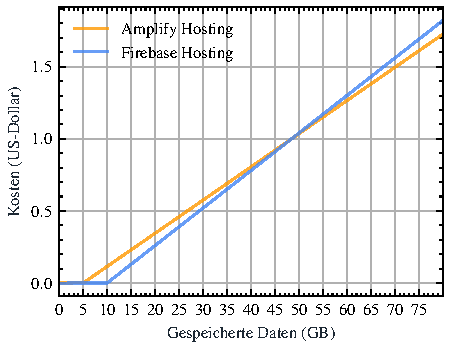
\includegraphics[width=6cm]{7_1_vergleich-cloud-kosten/hosting-stored-data.pdf} }}%
    \qquad
    \subfloat[\centering Übertragene Daten]{{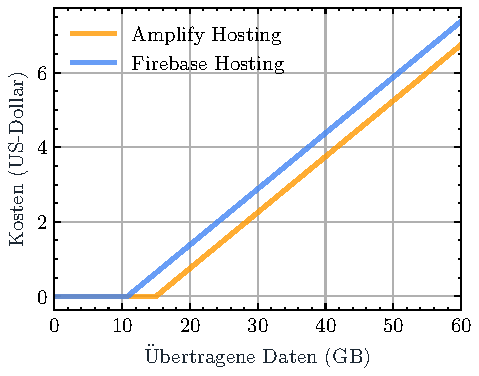
\includegraphics[width=6cm]{7_1_vergleich-cloud-kosten/hosting-transferred-data.pdf} }}%
    \caption{Kostenvergleich zwischen Amplify Hosting und Firebase Hosting}%
    \label{kostenvergleichHosting}%
\end{figure}

Amplify Hosting vs Firebase Hosting

Parameter:
- Gespeicherte Dateien
- Ausgelieferte Dateien

- Number of build minutes (nur AWS)


Amplify:
- Build minutes cost = Number of build minutes * 0,01 USD / min
- Data stored cost = Data stored per month GB * 0.023 USD / GB * mon
- Data served cost = Data served per month GB * 0.15 USD / GB * mon

Free tier:
5 GB stored per month
15 GB served per month

Firebase:
- Berechnung
    - Storage = $0.026/GB
    - Data transfer = $0.15/GB

Free tier:
- Storage 10 GB
- Data transfer: 10.8GB

\subsection{Serverless-Computing}

\begin{figure}
  \centering
  \subfloat[][\centering Ausführungszeit]{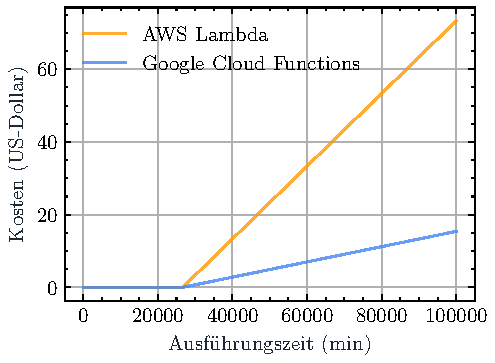
\includegraphics[width=.4\textwidth]{7_1_vergleich-cloud-kosten/functions-compute.pdf}}\quad
  \subfloat[][\centering Funktionsaufrufe]{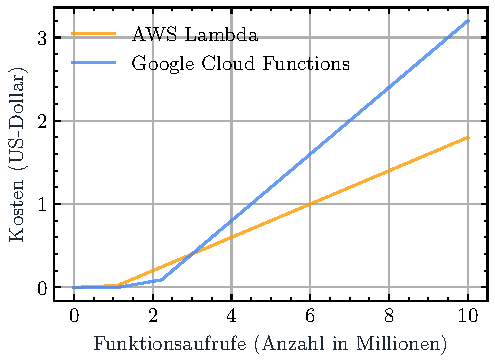
\includegraphics[width=.4\textwidth]{7_1_vergleich-cloud-kosten/functions-invocation.pdf}}\\
  \subfloat[][\centering Ausgehender Netzwerktransfer]{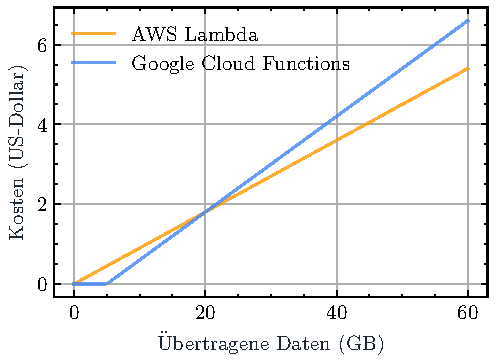
\includegraphics[width=.4\textwidth]{7_1_vergleich-cloud-kosten/functions-transfer.pdf}}\quad
  \caption{Kostenvergleich zwischen AWS Lambda und Google Cloud Functions}
  \label{kostenvergleichFunctions}
\end{figure}

AWS Lambda mit Cloud Functions

256MB

Lambda billed auf 1ms gerundet
Cloud Functions billed auf 100ms, daher ist der preis günstiger, da dadurch mehr gezahlt werden muss
Anhand von Beispiel darstellen

AWS Lambda (x86)
  - Compute Charges = 0.0000166667 USD pro GBs / 400,000 GB-seconds of compute time per month
  - Request Charges = 0,2 USD pro Millionen Request / one million free requests
  - Data Transfer Costs = APPSYNC Avg response size * Modifications * $0.09 USD /.GB

Cloud Functions (256MB)
  - Compute Time = 0.0000035 USD pro GBs (400,000 GB-seconds)
  - Invocations = $0.40 per Million requests (first 2m free)
  - Outbound Data (Egress) $0.12 pro GB, 5GB free ()

Da Lambda über AppSync ins Internet geht, werden hier die Preise von AppSync genutzt verglichen mit Cloud Functions.

x86 Price
Tier 2 Pricing bei Google Cloud
CPU skaliert mit der Memory automatisch mit
Cloud Functions berechnen auch die Build Minutes zum Bauen

\subsection{Storage}

\begin{figure}
  \centering
  \subfloat[][\centering Gespeicherte Daten]{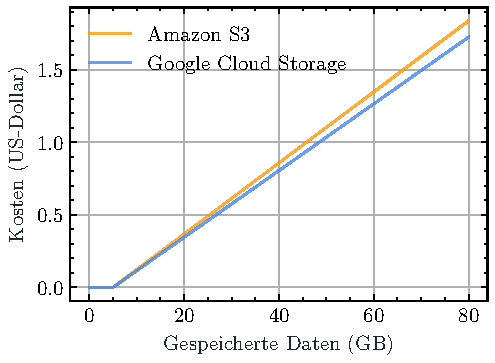
\includegraphics[width=.4\textwidth]{7_1_vergleich-cloud-kosten/storage-amount.pdf}}\quad
  \subfloat[][\centering Get-Anfragen]{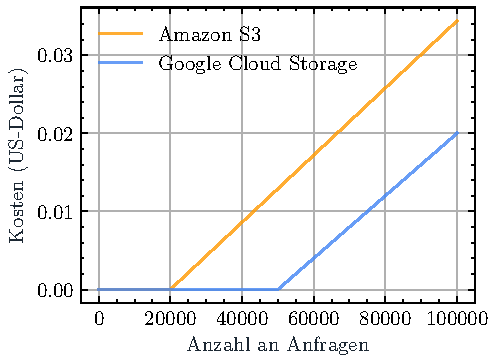
\includegraphics[width=.4\textwidth]{7_1_vergleich-cloud-kosten/storage-get.pdf}}\\
  \subfloat[][\centering Put/Post/List-Anfragen]{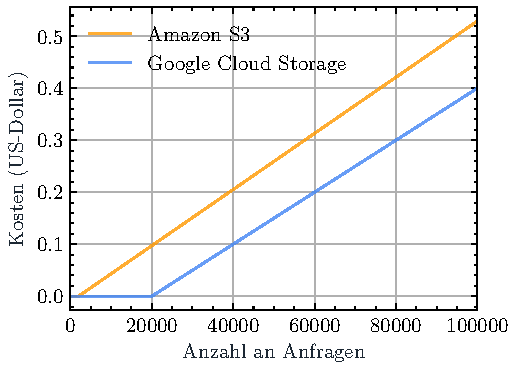
\includegraphics[width=.4\textwidth]{7_1_vergleich-cloud-kosten/storage-put.pdf}}\quad
  \subfloat[][\centering Ausgehender Netzwerktransfer]{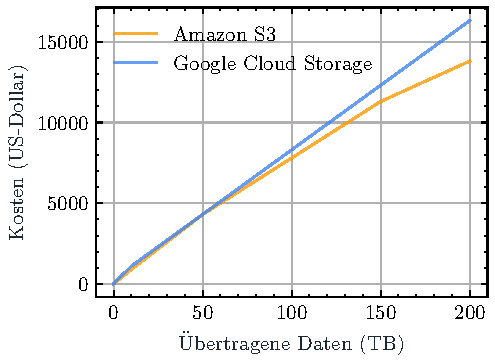
\includegraphics[width=.4\textwidth]{7_1_vergleich-cloud-kosten/storage-network.pdf}}
  \caption{Kostenvergleich zwischen Amazon S3 und Google Cloud Storage}
  \label{kostenvergleichStorage}
\end{figure}


AWS S3 mit Cloud Storage

S3

- Menge gespeicherter Daten
- Put, Post, List und Delete-Anfragen
- Get-Anfragen

Parameter
- S3 Standard Storage in GB
- PUT, COPY, POST, LIST Requests
- GET, SELECT Requests
- Inbound Data Transfer: Free
- Outbound Data Transfer: GB

Berechnung:
- S3 Standard Storage Costs: S3 Standard Storage in GB * 0.0245000000 USD
- S3 Standard PUT request costs: Number of PUT requests * 0.0000054 USD per request
- S3 Standard GET request costs: Number of GET requests * 0.00000043 USD per request
- Outbound Data Transfer:
    - 10240 GB x 0.09 USD per GB  (first 10TB)
    - 40960 GB x 0.085 USD per GB = 3481.60 USD (next 40TB)
    - 102400 GB x 0.07 USD per GB = 7168.00 USD (next 100TB)
    - 999846400 GB x 0.05 USD per GB = 49992320.00 USD (larger than 150TB)

Free tier: (für 12 Monate allerdings nur)
- 5 GB of Standard Storage
- 20,000 Get Requests
- 2,000 Put Requests

Ingress / Egress in beiden kostenlos

Cloud Storage (Standard Storage,
- Parameter
    - GB stored
    - Class A Operations: PUT, POST, LIST etc.
    - Class B Operations: GET
    - GB transferred
- Berechnung
    - Storage costs: $0.023 per GB / month
    - Class A = $0.05 per 10.000 Class A operations
    - Class B = $0.004 per 10.000 Class B operations
    - Transfer to Internet =  (Egress to Worldwide Destinations (excluding Asia & Australia) (per GB))
      - 0-1 TB $0.12
      - 1-10 TB	$0.11
      - 10+ TB $0.08

Free tier:
- 5GB storage
- 50k Class B
- 20K Class A
- 30 GB transfer


\subsection{Datenbank-Service}

DynamoDB mit Cloud Firestore

DynamoDB

Parameter:
- Data storage size in GB
- Average item size
- Writes
    - Standard writes vs Transactional writes: 100 / 0
    - Number of writes: 1000
- Reads
    - Eventually consistent vs Strongly vs Transactional: 100 / 0 / 0
    - Number of reads: 10 million per month
- On demand backup data storage

Free tier:
- 25 GB of Storage
- 25 provisioned Write Capacity Units (WCU)
- 25 provisioned Read Capacity Units (RCU)
- Enough to handle up to 200M requests per month.

Berechnung:
- Data storage costs: Data storage size * 0.306 USD
- Write costs: Number of writes * 0.000001525 USD
- Read costs: Number of reads x 1 strongly consistent portion x 1 read request units for strongly consistent reads x 25 read request units needed per item = 7,850,000,000.00 read request units for strongly consistent reads * 0.000000305 USD
- Backup storage costs: On demand backup data storage x 0.1224 USD



Cloud Firestore
- Parameter
    - GB stored
    - Document writes
    - Document reads
    - Document deletes
- Berechnung
    - Stored Data  = $0.117 per GB/ Month
    - Reads = $0.039/ 100.000 documents
    - Writes = $0.117 / 100.000 documents
    - Deletes = $0.013 / 100.000 documents
    - Transfer = ?

Free tier:
    Stored data	1 GiB
    Document reads	50,000 per day
    Document writes	20,000 per day
    Document deletes	20,000 per day
    Network egress	10 GiB per month


\subsection{Videokonvertierung}

\begin{figure}
  \centering
  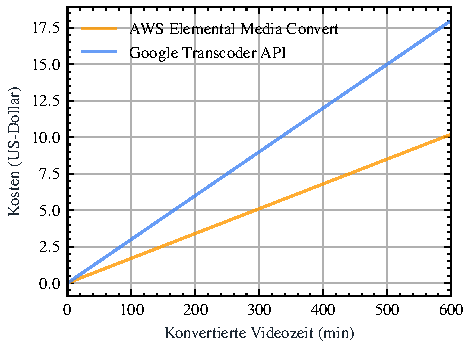
\includegraphics[width=0.75\columnwidth]{7_1_vergleich-cloud-kosten/transcoding.pdf}
  \caption{Kostenvergleich zwischen AWS Elemental Media Convert und Google Transcoder API}
  \label{KostenVideoTranscoding}
\end{figure}

AWS Elemental MediaConvert mit Google Transcoder API

AWS Elemental MediaConvert

Parameter:
- Tier: basic (Fix), Video-Codec: AVC, Single pass, HD, <= 30 FPS
- Output usage minutes per month

Berechnung:
- Outputs: Output usage minutes per month * 0.017 USD / minute


Google Transcoder API
- Parameter
    - Minutes HD conversion
- Berechnung
    - Price = Minutes * $0.030 USD / minute


\subsection{Zusammenfassung}

zusammenfassung aller dienste und wo welcher dienst günstiger ist

\subsection{Sonstige}

Zu beachten ist zuletzt, dass einige Dienste für \ac{AWS} Amplify benötigt werden, die in Firebase nicht vorhanden sind oder in beiden Diensten nicht abgerechnet werden.
\begin{description}
\item[User Management] Da die erweiterten Sicherheitsfunktionalitäten von \ac{AWS} Cognito nicht genutzt werden, ist dieser kostenfrei. Auch seitens Firebase gibt es für das User-Management keine extra Kosten für die Standardfunktionalität.
\item[Benachrichtigung von Diensten] Amazon EventBridge wird verwendet, um \ac{AWS} Lambda darüber zu benachrichtigen, dass ein Video erfolgreich konvertiert wurde. Der Dienst kostet pro 1 Millionen Custom Events \$ 1,00. In Firebase ist dafür kein zusätzlicher Dienst nötig.
\item[GraphQL] Aufgrund von Unterschieden in der Architektur nutzt \ac{AWS} Amplify mit AWS AppSync einen GraphQL-Server, während Firebase ohne einen solchen auskommt, da Funktionen direkt aus dem Frontend aufgerufen werden können. Bei \ac{AWS} entstehen dadurch Nutzungskosten von \$ 4,00 für 1 Millionen Queries oder Mutations. Außerdem entstehen Datentransferkosten. Diese sind allerdings schon durch die Netzwerkkosten aus \ac{AWS} Lambda abgedeckt.
\end{description}

\section{Preisbeispiele}

- Szenarien 1 2 3 ggf. auch nur eins

TODO: Nutzungsprofile für die Anwendung definieren, damit der vergleich einfacher ist